% !TEX root = _individual/adDerivation.tex

%%%%%%%%%%%%%%%%%%%%%%%%%%%%%%%%%%%%%%%%%%%%%%%%%%%%%%%%%%%%%%%%%%%%%%%%%%%%%%%%
\chapter{Anisotropic diffusion}\label{chap:adDerivation}

\newcommand{\Iv}{I_\mathrm{v}}
\newcommand{\Ibl}{I_\mathrm{bl}}
\newcommand{\Iil}{I_\mathrm{il}}

Existing radiation transport methods, the most common of which were presented
in the last chapter, approximate the angular dependence of the intensity each
in a different way. The crudest of these, diffusion, has only one unknown
$\phi$ at each point in space and time; the more complex such as \SN\ have many
unknowns, leading to greater accuracy but greater computer run time and memory
usage. In this chapter, we derive a new anisotropic diffusion method, which
approximates the intensity in such a way as to retain an arbitrary amount of
anisotropy (like a true transport method), while solving for a single unknown
(like a diffusion method).

The previous work in anisotropic diffusion has only considered steady-state,
linear problems in an infinite medium \cite{Lar2009c,Mor2007}. The new
derivation of
the anisotropic diffusion approximation presented in this chapter provides a
theoretical basis for using AD in time-dependent, nonlinear problems, and it
also addresses boundary conditions for the AD method.

%%%%%%%%%%%%%%%%%%%%%%%%%%%%%%%%%%%%%%%%%%%%%%%%%%%%%%%%%%%%%%%%%%%%%%%%%%%%%%%%
\section{Linear time-dependent derivation}

In this section, we use an asymptotic analysis to derive the anisotropic
diffusion approximation in a linear, time-dependent, finite problem. To apply
the resulting equations to nonlinear thermal radiative transfer, we appeal to
both the linear formulation of the semi-implicit method (REF) and a very similar
asymptotic analysis of the equilibrium radiation diffusion approximation in
Ref.~\cite{Lar1983a}.

We begin with a linear, time-dependent transport problem with specified incident
boundaries and isotropic scattering. The transport equation is
\begin{subequations} \label{eqs:tdTransport}
\begin{multline} \label{eq:tdTransportVol}
  \frac{1}{c}\pder{I}{t}(\vec{x},\vec{\Omega},t)
  + \vec{\Omega}\vd \grad I(\vec{x},\vec{\Omega},t)
  + \sigma(\vec{x}) I(\vec{x},\vec{\Omega},t)
  \\ = \frac{\sigma_s(\vec{x})}{4\pi}
  \int_{4\pi} I(\vec{x},\vec{\Omega}',t) \ud \Omega'
  + \frac{q(\vec{x},t)}{4\pi}
  \,, \quad \vec{x}\in V,\ \vec{\Omega}\in4\pi,\ t \ge 0.
\end{multline}
The boundary condition is specified
for incident directions:
\begin{equation} \label{eq:tdTransportBndy}
  I(\vec{x},\vec{\Omega},t) = I^b(\vec{x},\vec{\Omega},t) \,,
  \quad \vec{x}\in \partial V ,\ \vec{\Omega}\vd \vec{n} < 0,\ t > 0,
\end{equation}
and the initial condition is
\begin{equation} \label{eq:tdTransportInit}
  I(\vec{x},\vec{\Omega},0) = I^i(\vec{x},\vec{\Omega}) \,,
  \quad \vec{x}\in V ,\ \vec{\Omega} \in 4\pi.
\end{equation}
\end{subequations}

Because this transport equation is linear, we can write its solution as the
superposition of three distinct transport solutions:
\begin{equation}\label{eq:tdSuperimposition}
  I(\vec{x},\vec{\Omega},t)
  \equiv \Iv(\vec{x},\vec{\Omega},t)
  + \Ibl(\vec{x},\vec{\Omega},t)
  + \Iil(\vec{x},\vec{\Omega},t)\,.
\end{equation}
Here, $\Iv$ is an ``interior'' solution valid many mean free paths away from
the exterior problem boundary and many free times away from $t=0$, $\Ibl$ is a
``boundary layer'' solution that decays rapidly away from the exterior boundary,
and $\Iil$ is an ``initial layer'' that decays rapidly away from $t=0$.

\begin{figure}[htb]
  \centering
  %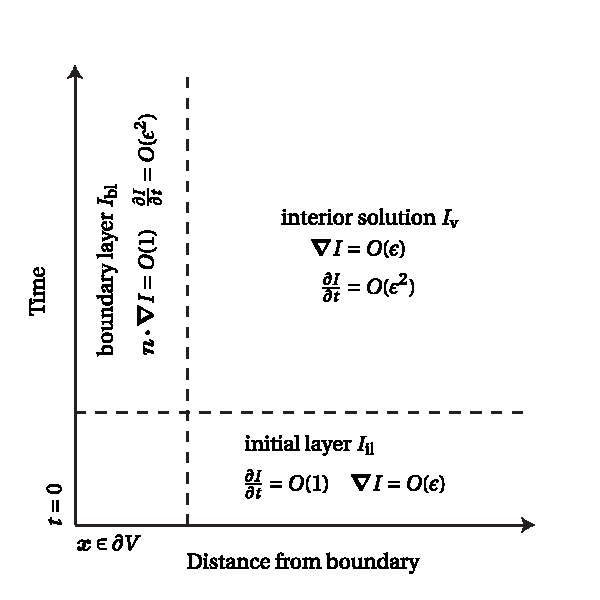
\includegraphics{layers}
  \caption{Depiction of interior, boundary layer, and initial layer of a
  transport problem.}
  \label{fig:layers}
\end{figure}

Our goal is to develop an approximation to $\Iv$ that satisfies the transport
equation in some asymptotic limit, and then use the boundary and initial layer
equations to ``match'' the interior solution to the transport solution on the
boundary and at the initial time.

%%%%%%%%%%%%%%%%%%%%%%%%%%%%%%%%%%%%%%%%%%%%%%%%%%%%%%%%%%%%%%%%%%%%%%%%%%%%%%%%
\subsection{Interior solution}

The interior transport equation accounts for the extraneous source term, but
it has no initial or boundary conditions, as it is only valid away from the
boundary and initial layer:
\begin{equation} \label{eq:tdVol}
  \frac{1}{c}\pder{\Iv}{t}(\vec{x},\vec{\Omega},t)
  + \vec{\Omega}\vd \grad \Iv(\vec{x},\vec{\Omega},t)
  + \sigma(\vec{x}) \Iv(\vec{x},\vec{\Omega},t)
  = \frac{\sigma_s(\vec{x})}{4\pi}
  \phi(\vec{x},t) + \frac{q(\vec{x},t)}{4\pi} \,.
\end{equation}
Here, we have defined
\begin{equation} \label{eq:tdPhi}
  \phi(\vec{x}) \equiv \int_{4\pi} \Iv(\vec{x}, \vec{\Omega},t) \ud \Omega\,,
\end{equation}
which is the \emph{interior} scalar intensity. We write Eq.~\eqref{eq:tdVol} as
\begin{equation*}
  \left[ \frac{1}{c}\pder{}{t}
  + \vec{\Omega}\vd \grad
  + \sigma \right] \Iv
  = \frac{\sigma_s}{4\pi}
  \phi + \frac{q}{4\pi} \,.
\end{equation*}

Taking the zeroth angular moment of Eq.~\eqref{eq:tdVol} gives a conservation
equation in the interior,
\begin{equation} \label{eq:loVol}
\frac{1}{c} \pder{\phi}{t} (\vec{x}, t)
  + \grad \vd\vec{F}(\vec{x}, t)
  + \sigma(\vec{x}) \phi(\vec{x}, t)
 = \sigma_s(\vec{x}) \phi(\vec{x},t) + q(\vec{x},t)\,.
\end{equation}
Adding $\vec{\Omega}\vd \grad \phi$ to both sides of Eq.~\eqref{eq:loVol} and
multiplying the resulting equation by $\frac{1}{4\pi}$, we obtain
\begin{align*}
  \left[ \frac{1}{c}\pder{}{t}
  + \vec{\Omega}\vd \grad
  + \sigma \right]
  \left( \frac{1}{4\pi} \phi \right)
  = \frac{\sigma_s}{4\pi}
  \phi + \frac{q}{4\pi} - \frac{1}{4\pi} \grad \vd\vec{F} 
  + \frac{1}{4\pi} \vec{\Omega}\vd \grad \phi\,.
\end{align*}
Subtracting this equation from Eq.~\eqref{eq:tdVol} cancels the isotropic source
and scattering term on the right-hand side, yielding the following equation:
\begin{equation}\label{eq:capPsiVol}
  \left[ \frac{1}{c}\pder{}{t}
  + \vec{\Omega}\vd \grad
  + \sigma \right]
   \left( \Iv
  - \frac{1}{4\pi} \phi \right)
  = \frac{1}{4\pi} \grad \vd\vec{F} -
  \frac{1}{4\pi} \vec{\Omega}\vd \grad \phi\,.
\end{equation}

At this point, we apply an asymptotic scaling typical of a diffusive regime.
We make an ansatz that the spatial gradients are weak, the speed of light is
large, and the solution is mildly (but not necessarily linearly) anisotropic:
\begin{align} \label{eq:ansatz}
  \sigma &= O(1), &
  \phi &= O(1), &
  \vec{F} &= O(\epsilon), &
  \grad &= O(\epsilon), &
  \pder{}{t} &= O(\epsilon^2) \,.
\end{align}
These scalings are the same as in an asymptotic derivation of the standard
diffusion equation \cite{Lar1975,Mor2000}. Applying them to
Eq.~\eqref{eq:capPsiVol} gives
\begin{equation*}
  \left[\vec{\Omega}\vd \grad
  + \sigma + O(\epsilon^2) \right]
   \left( \Iv
  - \frac{1}{4\pi} \phi \right)
  = - \frac{1}{4\pi} \vec{\Omega}\vd \grad \phi + O(\epsilon^2)\,.
\end{equation*}
Now we discard the $O(\epsilon^2)$ terms:
\begin{equation*}
  \left[\vec{\Omega}\vd \grad  + \sigma \right]
   \left( \Iv
  - \frac{1}{4\pi} \phi \right)
  = - \frac{1}{4\pi} \vec{\Omega}\vd \grad \phi \,.
\end{equation*}
Formally inverting the bracketed operator on the left-hand side, we obtain an
approximate expression for the intensity in the interior:
\begin{equation}\label{eq:tdVolApprox1}
  \Iv = \frac{1}{4\pi} \phi - 
  \left[\vec{\Omega}\vd \grad  + \sigma \right]\inv
  \left( \frac{1}{4\pi} \vec{\Omega}\vd \grad \phi \right)\,.
\end{equation}

The inverted differential operator is an integral transport operator
\cite{Pri2010}:
\begin{subequations} \label{eqs:inverseTransport}
  \begin{align} \label{eq:inverseTransportFull}
  \begin{split}
    \left[\vec{\Omega}\vd \grad  + \sigma \right]\inv
    \hat Q(\vec{x}, \vec{\Omega})
    &=
     \int_{0}^{\infty}
    \hat Q(\vec{x} - s \vec{\Omega}, \vec{\Omega}, t)
    \eexp^{ -\tau(\vec{x}, \vec{x} - s \vec{\Omega})}
    \ud s
\,.
  \end{split}
  \end{align}
  Here, the optical distance between points $\vec{x}$ and
  $\vec{x}'$ along the direction $\vec{\Omega} = (\vec{x}'-
  \vec{x})/\norm{\vec{x}'-\vec{x}}$ is 
  \begin{equation} \label{eq:fullTauDefinition}
    \tau(\vec{x}, \vec{x}') = \int_{0}^{\norm{\vec{x} -
    \vec{x}'}} \sigma(\vec{x}-s\vec{\Omega}) \ud s \,.
  \end{equation}
\end{subequations}

Thus Eq.~\eqref{eq:tdVolApprox1} for the interior intensity is a function of the
nonlocal unknown scalar flux:
\begin{equation*}
  \Iv(\vec{x},\vec{\Omega},t) = \frac{1}{4\pi} \phi(\vec{x},t) - 
     \int_{0}^{\infty}
    \frac{1}{4\pi} \vec{\Omega}\vd \grad \phi(\vec{x} - s \vec{\Omega}, \vec{\Omega}, t)
    \eexp^{ -\tau(\vec{x}, \vec{x} - s \vec{\Omega})}
    \ud s \,.
\end{equation*}
To simplify, we use the assumption that spatial gradients are weak (see
Eq.~\eqref{eq:ansatz}) to expand $\phi$ in a Taylor series about the local
point:
\begin{equation} \label{eq:taylorPhi}
  \phi(\vec{x} - s \vec{\Omega}, t)
  = \phi(\vec{x},t) - s\vec{\Omega} \vd
  \grad\phi (\vec{x}, t) + O(\epsilon^2) = \phi(\vec{x},t) +
  O(\epsilon) \,.
\end{equation}


\begin{align}\nonumber
  \Iv(\vec{x},\vec{\Omega},t) &= \frac{1}{4\pi} \phi(\vec{x},t) - 
     \int_{0}^{\infty}
    \frac{1}{4\pi} \vec{\Omega}\vd \grad \phi(\vec{x} - s \vec{\Omega}, \vec{\Omega}, t)
    \eexp^{ -\tau(\vec{x}, \vec{x} - s \vec{\Omega})}
    \ud s
\\
  &= \int_{0}^{\infty}
    \left[ -\frac1{4\pi}\vec{\Omega}\vd \grad \phi(\vec{x},t) + O(\epsilon^2) \right]
    \eexp^{ -\tau(\vec{x}, \vec{x} - s \vec{\Omega})}
    \ud s
  \\ \nonumber
  &= - \int_{0}^{\norm{\vec{x} - \vec{x}_b}}
    \left[ \frac1{4\pi}\right]
    \eexp^{ -\tau(\vec{x}, \vec{x} - s \vec{\Omega})} \ud s \,
    \vec{\Omega}\vd \grad \phi(\vec{x},t)
  \\\label{eq:streamingApprox}
  &= - \lopinv{v}{ \frac1{4\pi} } \vec{\Omega}\vd \grad \phi(\vec{x},t)
  \,.
\end{align}

To simplify, we expand $\phi$ in a Taylor series about the local
point:
\begin{equation} \label{eq:taylorPhi}
  \phi(\vec{x} - s \vec{\Omega}, t)
  = \phi(\vec{x},t) - s\vec{\Omega} \vd
  \grad\phi (\vec{x}, t) + O(\epsilon^2) = \phi(\vec{x},t) +
  O(\epsilon) \,.
\end{equation}
Here we have used the assumption from Eq.~\eqref{eq:ansatz} that gradients are
$O(\epsilon)$, giving
\begin{equation*}
  \grad \phi(\vec{x}-s\vec{\Omega},t)
  = \grad \phi(\vec{x},t) + O(\epsilon^2)\,,
\end{equation*}
since $\grad \phi=O(\epsilon)$. This approximates Eq.~\eqref{eq:tdVolApprox1} as
\begin{equation*}
  \Iv = \frac{1}{4\pi} \phi - 
  \left[\vec{\Omega}\vd \grad  + \sigma \right]\inv
  \left( \frac{1}{4\pi}\right) \left( \vec{\Omega}\vd \grad \phi \right)
  + O(\epsilon^2) \,,
\end{equation*}
which we write as
\begin{equation}\label{eq:tdVolApprox2}
  \Iv(\vec{x},\vec{\Omega},t)
  = \frac{1}{4\pi} \phi (\vec{x},t)
  - f(\vec{x}, \vec{\Omega})\vec{\Omega}\vd \grad \phi(\vec{x},t)\,,
\end{equation}
where we have defined
\begin{equation*}
  f(\vec{x},\vec{\Omega}) = \left[\vec{\Omega}\vd \grad  + \sigma \right]\inv
  \left( \frac{1}{4\pi}\right) \,,
\end{equation*}
which is the solution to the following differential transport equation:
\begin{equation} \label{eq:fFullVol}
  \vec{\Omega}\vd \grad f(\vec{x}, \vec{\Omega})
  + \sigma(\vec{x}) f (\vec{x}, \vec{\Omega})
= \frac{1}{4\pi} \,.
\end{equation}

Taking the first angular moment of Eq.~\eqref{eq:tdVolApprox2} gives an
approximate expression for the radiation flux in the interior:
\begin{align} \nonumber
  \vec{F}(\vec{x},t) &= \int_{4\pi} \vec{\Omega} \Iv(\vec{x},\vec{\Omega},t)
  \ud\Omega
  \\ \nonumber
  &= - \left[ \int_{4\pi} \vec{\Omega} \vec{\Omega} f(\vec{x}, \vec{\Omega}) \ud\Omega
  \right] \vd \grad \phi(\vec{x},t)
  \\ \label{eq:anisotropicFicks}
  &= - \Dtens(\vec{x}) \vd \grad \phi(\vec{x},t) \,.
\end{align}
This resembles ``Fick's law,'' but instead of a scalar diffusion
\emph{coefficient},
the anisotropic diffusion method has a diffusion \emph{tensor}, $\Dtens$, the
second angular moment of $f$:
\begin{equation}\label{eq:dDefinition}
  \Dtens(\vec{x}) \equiv \int_{4\pi} \vec{\Omega} \vec{\Omega}
  f(\vec{x}, \vec{\Omega}) \ud\Omega \,.
\end{equation}

Because of the approximations made in developing Eq.~\eqref{eq:tdVolApprox2},
$\phi$ no longer satisfies the exact transport solution. Instead, like Fick's
law, the first-order accurate approximation to the radiation flux is substituted
into the low-order conservation equation~\eqref{eq:loVol} to yield an
anisotropic diffusion equation that $\phi$ satisfies in the interior:
\begin{equation} \label{eq:tdVolDiffusion}
\frac{1}{c} \pder{\phi}{t} (\vec{x}, t)
  - \grad \vd \Dtens(\vec{x}) \vd \grad \phi(\vec{x},t)
  + \sigma_a(\vec{x}) \phi(\vec{x}, t)
 = q(\vec{x},t)\,.
\end{equation}
Here we use the absorption opacity $\sigma_a = \sigma - \sigma_s$.

The anisotropic diffusion approximation to the interior solution $I_v$
comprises \textsl{(i)} the transport equation~\eqref{eq:fFullVol} for $f$,
\textsl{(ii)} the definition in Eq.~\eqref{eq:dDefinition} of the diffusion
tensor $\Dtens$, and \textsl{(iii)} the anisotropic diffusion
equation~\eqref{eq:tdVolDiffusion}.

%%%%%%%%%%%%%%%%%%%%%%%%%%%%%%%%%%%%%%%%%%%%%%%%%%%%%%%%%%%%%%%%%%%%%%%%%%%%%%%%
\subsection{Initial layer solution}

The initial layer consists of a transport problem near the initial time $t=0$,
where the time derivatives are not assumed to be $O(\epsilon^2)$ but rather
$O(1)$. It is defined in the spatial interior of the problem, where
spatial gradients are still assumed to be $O(\epsilon)$, and the exterior
problem boundary is not considered. The initial layer transport problem
complements the interior transport equation~\eqref{eq:tdVol}, so it does not
have a source term:
\begin{subequations} \label{eqs:tdInitVol}
\begin{equation} \label{eq:tdInit}
  \frac{1}{c}\pder{\Iil}{t}(\vec{x},\vec{\Omega},t)
  + \vec{\Omega}\vd \grad \Iil(\vec{x},\vec{\Omega},t)
  + \sigma(\vec{x}) \Iil(\vec{x},\vec{\Omega},t)
  = \frac{\sigma_s(\vec{x})}{4\pi}
  \int_{4\pi} \Iil(\vec{x},\vec{\Omega}',t) \ud \Omega' \,.
\end{equation}
Because it is defined for times close to $t=0$, it accounts for the initial
condition in Eq.~\eqref{eq:tdTransportInit} using the superposition
equation~\eqref{eq:tdSuperimposition}. We have set $\Ibl=0$ because the
transport equation is defined only in the spatial interior where the boundary
layer has decayed. Thus the relation between the initial layer's initial
condition and the true initial condition is:
\begin{equation}\label{eq:tdInitInit}
 \Iv(\vec{x},\vec{\Omega},0) + \Iil(\vec{x},\vec{\Omega},0)
 = I^i(\vec{x},\vec{\Omega})\,.
\end{equation}
Furthermore, by construction we demand that its solution tend to zero for
increasing $t$:
\begin{equation} \label{eq:tdInitLimit}
  \lim_{t\to\infty} \Iil(\vec{x},\vec{\Omega},t) \,.
\end{equation}
\end{subequations}

A formal asymptotic analysis for the initial layer explicitly sets
$\grad\to\epsilon\grad$, expands $\Iil$ in powers of $\epsilon$, and matches it
with the asymptotic interior solution $\Iv$. A simpler but effectively
equivalent procedure is to demand that the initial layer contain no particles
at the initial time:
\begin{equation*}
  \int_{4\pi} \Iil(\vec{x}, \vec{\Omega}, 0) \ud \Omega = 0\,.
\end{equation*}
Integrating Eq.~\eqref{eq:tdInitInit} over all angles and applying this demand, we
obtain a relation between the interior solution and the transport initial
condition
\begin{align*}
\int_{4\pi} \Iv(\vec{x},\vec{\Omega},0) \ud\Omega
+ \int_{4\pi} \Iil(\vec{x},\vec{\Omega},0) \ud\Omega
 &= \int_{4\pi} I^i(\vec{x},\vec{\Omega}) \ud\Omega
 \\
 \int_{4\pi} \left[ \frac{\phi(\vec{x},0)}{4\pi} - f(\vec{x},\vec{\Omega})
 \vec{\Omega}\vd \grad \phi(\vec{x},0) ) \right] \ud\Omega
 + 0 &= \phi^i(\vec{x})
\end{align*}

%%%%%%%%%%%%%%%%%%%%%%%%%%%%%%%%%%%%%%%%%%%%%%%%%%%%%%%%%%%%%%%%%%%%%%%%%%%%%%%%
%%%%%%%%%%%%%%%%%%%%%%%%%%%%%%%%%%%%%%%%%%%%%%%%%%%%%%%%%%%%%%%%%%%%%%%%%%%%%%%%
%%%%%%%%%%%%%%%%%%%%%%%%%%%%%%%%%%%%%%%%%%%%%%%%%%%%%%%%%%%%%%%%%%%%%%%%%%%%%%%%
%%%%%%%%%%%%%%%%%%%%%%%%%%%%%%%%%%%%%%%%%%%%%%%%%%%%%%%%%%%%%%%%%%%%%%%%%%%%%%%%
%%%%%%%%%%%%%%%%%%%%%%%%%%%%%%%%%%%%%%%%%%%%%%%%%%%%%%%%%%%%%%%%%%%%%%%%%%%%%%%%
\section{OLD STUFF}

Here, $\vec{\Omega}_r$ is the reflected angle on a boundary surface with outward
normal $\vec{n}$:
\begin{equation} \label{eq:reflection}
  \vec{\Omega}_r = \vec{\Omega} - 2(\vec{\Omega} \vd \vec{n}) \vec{n}\,.
\end{equation}

%%%%%%%%%%%%%%%%%%%%%%%%%%%%%%%%%%%%%%%%
\subsection{Approximating the streaming integral term}\label{sec:adStreaming}
The streaming term in Eq.~\eqref{eq:approxPsi1} is (see
Eq.~\eqref{eq:inverseTransportFull}):
\begin{align*}
- \lopinv{v}{\frac{1}{4\pi} \vec{\Omega}\vd \grad \phi(\vec{x}, t)}
  &= \int_{0}^{\norm{\vec{x} - \vec{x}_b}}
    \left[ -\frac1{4\pi}\vec{\Omega}\vd \grad \phi(\vec{x} - s \vec{\Omega},
    t-s/c)
    \right]
    \eexp^{ -\tau(\vec{x}, \vec{x} - s \vec{\Omega})}
    \ud s\,.
\end{align*}
This integral describes the contribution from the volumetric source  along
$\vec{\Omega}$, evaluated at a prior
point in time ($t-s/c$, the point along $s$ at which a particle would travel
to $\vec{x}$ at time $t$), attenuated by the medium along the way by collisions.

We now make our first approximation by expanding the distant $\phi(\vec{x} - s
\vec{\Omega}, t-s/c)$ about the local $\phi(\vec{x}, t)$ using
Eq.~\eqref{eq:taylorPhi}. Thus,
\begin{equation*}
  \grad \phi(\vec{x} - s \vec{\Omega}, t-s/c)
  = \grad \left[ \phi(\vec{x}, t) + O(\epsilon) \right]
  = \grad \phi(\vec{x}, t) + O(\epsilon^2).
\end{equation*}
The expansion is a good approximation if $\phi$ is smooth.

We can now move the unknown $\phi$ outside the integral,
because it is no longer a function of $s$:
\begin{align}\nonumber
- \lopinv{v}{\frac{1}{4\pi} \vec{\Omega}\vd \grad \phi(\vec{x}, t)}
  &\approx \int_{0}^{\norm{\vec{x} - \vec{x}_b}}
    \left[ -\frac1{4\pi}\vec{\Omega}\vd \grad \phi(\vec{x},t) \right]
    \eexp^{ -\tau(\vec{x}, \vec{x} - s \vec{\Omega})}
    \ud s
  \\\nonumber
  &= - \int_{0}^{\norm{\vec{x} - \vec{x}_b}}
    \left[ \frac1{4\pi}\right]
    \eexp^{ -\tau(\vec{x}, \vec{x} - s \vec{\Omega})} \ud s \,
    \vec{\Omega}\vd \grad \phi(\vec{x},t)
  \\\label{eq:streamingApprox}
  &= - \lopinv{v}{ \frac1{4\pi} } \vec{\Omega}\vd \grad \phi(\vec{x},t)
  \,.
\end{align}
Thus the function of nonlocal unknowns has been approximated by a nonlocal known, the
$\lopinv{v}{\cdot}$ term, and a local unknown, $\phi(\vec{x},t)$.

%%%%%%%%%%%%%%%%%%%%%%%%%%%%%%%%%%%%%%%%
\subsection{Anisotropic diffusion approximation to \texorpdfstring{$\Psi$}{Psi}}
Substituting Eqs.~\eqref{eq:streamingApprox},~\eqref{eq:bndyApprox},
and~\eqref{eq:reflApprox} into Eq.~\eqref{eq:approxPsi1} gives a nearly complete
approximation to the anisotropic component of the angular intensity,
$\Psi=I-\frac{1}{4\pi}\phi$:
\begin{align} \nonumber
  \tilde\Psi
  &\approx 
- \lopinv{b}{\zeta}_{\partial V} \vec{\Omega}\vd \grad \phi
- \lopinv{b}{f(\vec{\Omega}_r)}_{\partial V_r}
  \vec{\Omega}\vd \grad \phi
- \lopinv{v}{\frac{1}{4\pi}}  \vec{\Omega}\vd \grad \phi
\\ \label{eq:approxPsi2}
  \tilde\Psi &= 
- \left\{ \lopinv{b}{\zeta}_{\partial V} 
+ \lopinv{b}{f(\vec{\Omega}_r)}_{\partial V_r}
+ \lopinv{v}{\frac{1}{4\pi}} \right\} \vec{\Omega}\vd \grad \phi
\\ \label{eq:approxPsi3}
\tilde\Psi(\vec{x}, \vec{\Omega}, t) &= - f(\vec{x}, \vec{\Omega})
\vec{\Omega}\vd \grad \phi(\vec{x}, t)\,.
\end{align}

Here, we have defined
\begin{equation*}
  f(\vec{x}, \vec{\Omega})
  \equiv \lopinv{b}{\zeta}_{\partial V} 
+ \lopinv{v}{\frac{1}{4\pi}}\,,
\end{equation*}
which is an integral transport equation [see Eqs.~\eqref{eqs:inverseTransport}].
Converting the integral transport equation to a differential
transport equation shows $f$ to be the solution to a purely absorbing transport
problem with a uniform, isotropic unit source:
\begin{subequations} \label{eqs:fFull}
  \begin{equation} \label{eq:fFullVol}
    \vec{\Omega}\vd \grad f(\vec{x}, \vec{\Omega})
    + \sigma f (\vec{x}, \vec{\Omega})
  = \frac{1}{4\pi} \,, \quad x \in V,\ \vec{\Omega} \in 4\pi\,,
  \end{equation}
with to-be-determined boundary conditions where the incident radiation is specified,
\begin{equation} \label{eq:fFullBndy}
  f(\vec{x}, \vec{\Omega}) = \zeta(\vec{x}, \vec{\Omega}) \,,
 \quad \vec{x} \in \partial V, \ \vec{\Omega} \vd \vec{n} < 0\,.
\end{equation}
  and with reflecting boundary conditions where the physical problem is
  reflecting,
\begin{equation} \label{eq:fFullRefl}
  f(\vec{x}, \vec{\Omega}) = f(\vec{x}, \vec{\Omega}_r) \,,
 \quad \vec{x} \in \partial V_r, \ \vec{\Omega} \vd \vec{n} < 0\,.
\end{equation}
\end{subequations}

Note that the transport equation is steady-state because $\frac{1}{c}\pder{}{t}=
O(\epsilon^2)$. Accordingly, $\zeta$ is restricted to a function constant within
the time step.

%%%%%%%%%%%%%%%%%%%%%%%%%%%%%%%%%%%%%%%%
\subsection{Approximate radiation flux}
Now we have an equation for $\tilde\Psi(\vec{x}, \vec{\Omega}, t)$ as a
separable
function of this simple transport equation $f(\vec{x}, \vec{\Omega})$ and the
scalar intensity $\phi(\vec{x},t)$.
We desire a simple low-order equation that provides a closure for the unknown
radiation flux $\vec{F}(\vec{x},t)$ in the radiation conservation
equation~\eqref{eq:loVol}.

We use the property from Eq.~\eqref{eq:capPsiFirst}
that the first moment of $\Psi$ is the flux $\vec{F}$. Operating on 
Eq.~\eqref{eq:approxPsi3} by $\int_{4\pi} \vec{\Omega} (\cdot) \ud\Omega$, we
obtain the following simple expression:
\begin{align} \nonumber
  \vec{F}(\vec{x}, t)
  &= \int_{4\pi} \vec{\Omega} \tilde \Psi(\vec{x}, \vec{\Omega}, t) \ud\Omega
  \\ \nonumber
  &= 
  - \left[ \int_{4\pi} \vec{\Omega} \vec{\Omega} f(\vec{x}, \vec{\Omega})
  \ud\Omega \right]
  \vd \grad \phi(\vec{x},t)
  \\ \label{eq:anisotropicFicks}
  &= - \Dtens(\vec{x}) \vd \grad \phi(\vec{x},t) \,.
\end{align}
This resembles ``Fick's law,'' but instead of a scalar diffusion
\emph{coefficient},
the anisotropic diffusion method has a diffusion \emph{tensor}, $\Dtens$, the
second angular moment of $f$:
\begin{equation}\label{eq:dDefinition}
  \Dtens(\vec{x}) \equiv \int_{4\pi} \vec{\Omega} \vec{\Omega}
  f(\vec{x}, \vec{\Omega}) \ud\Omega \,.
\end{equation}

Like Fick's law, Eq.~\eqref{eq:anisotropicFicks} is substituted into
the low-order conservation equation~\eqref{eq:loVol}.
However, this ``Fick's law'' does not directly describe the behavior of $f$ or
$\phi$ at the boundary. For boundary conditions that relate $\phi$, $f$, and
$\zeta$, we turn to the boundary layer equations~\eqref{eqs:blCapPsi}.

%%%%%%%%%%%%%%%%%%%%%%%%%%%%%%%%%%%%%%%%
\subsection{Incident boundary condition}\label{sec:zeta}

The unknown function $\zeta(\vec{x}, \vec{\Omega})$ that lives on the boundary
is a degree of freedom introduced at the beginning of the anisotropic
diffusion derivation. The replacement of $\Psi_b$ with $-\zeta \vec{\Omega} \vd
\grad \phi$ allowed us to formulate a specified boundary condition
such that the effect of incident radiation boundaries could be embedded in the
anisotropic diffusion tensor $\Dtens$.

To make use of this degree of freedom, we decide to enforce on the boundary the
truth from Eq.~\eqref{eq:capPsiZeroth},
\begin{equation*}
  \int_{4\pi} \Psi(\vec{x}, \vec{\Omega}, t) \ud\Omega
  = 0 \,.
\end{equation*}
Note that our approximate $\tilde\Psi$ defined in Eq.~\eqref{eq:approxPsi3}
does not generally satisfy this identity:
\begin{align*}
  0
&\qeq \int_{4\pi} \tilde\Psi(\vec{x}, \vec{\Omega}, t) \ud\Omega
\\
0 &\qeq \int_{4\pi} \left[ - f(\vec{x}, \vec{\Omega}) \vec{\Omega}
\vd \grad \phi(\vec{x}, t)\right]
\ud\Omega
\\
\vec{0} &\qeq \int_{4\pi} \vec{\Omega} f(\vec{x}, \vec{\Omega})\ud\Omega \,.
\end{align*}
However, on exterior source boundaries, because $\zeta$ is defined for incident
directions and $f$ is known for exiting directions, we can choose $\zeta$ such
that this identity holds true under certain conditions.

Returning to the description of $f$ on an incident boundary in
Eq.~\eqref{eq:fFullBndy}, we write
\begin{align*}
  \int_{4\pi} \vec{\Omega} f(\vec{x}, \vec{\Omega})\ud\Omega
  &= \int_{\vec{\Omega} \vd \vec{n} < 0}
  \vec{\Omega} \zeta(\vec{x}, \vec{\Omega})\ud\Omega
  + \int_{\vec{\Omega} \vd \vec{n} > 0}
  \vec{\Omega} f(\vec{x}, \vec{\Omega})\ud\Omega\,.
\end{align*}
Now we set the left hand side to zero to satisfy $\int_{4\pi} \tilde\Psi \ud\Omega = 0$:
\begin{align}
  \label{eq:zetaCondition1}
  \int_{\vec{\Omega} \vd \vec{n} < 0}
  \vec{\Omega} \zeta(\vec{x}, \vec{\Omega})\ud\Omega
  &= -\int_{\vec{\Omega} \vd \vec{n} > 0}
  \vec{\Omega} f(\vec{x}, \vec{\Omega})\ud\Omega \,.
  \\ 
  \intertext{Making the substitution $\vec{\Omega}\to -\vec{\Omega}$ on the
  right hand side yields}
  \label{eq:zetaCondition2}
  \int_{\vec{\Omega} \vd \vec{n} < 0}
  \vec{\Omega} \zeta(\vec{x}, \vec{\Omega})\ud\Omega
  &= \int_{\vec{\Omega} \vd \vec{n} < 0}
  \vec{\Omega} f(\vec{x}, -\vec{\Omega})\ud\Omega \,.
\end{align}

If $f(\vec{\Omega})$ is azimuthally symmetric about $\vec{n}$, then $f$ is only
a function of the cosine angle between $\vec{\Omega}$ and $\vec{n}$:
\begin{equation*}
f(\vec{\Omega}) = \hat f( \vec{\Omega} \vd \vec{n})\,.
\end{equation*}
Now recall the definition of a reflecting boundary from
Eq.~\eqref{eq:reflection},
\begin{equation*}
  \vec{\Omega}_r = \vec{\Omega} - 2(\vec{\Omega} \vd \vec{n}) \vec{n}\,.
\end{equation*}
Dotting the reflected vector with the normal vector $\vec{n}$,
\begin{equation*}
  \vec{\Omega}_r \vd \vec{n}
  = \vec{\Omega} \vd \vec{n} - 2(\vec{\Omega} \vd \vec{n}) \vec{n}\vd \vec{n}
  = - \vec{\Omega} \vd \vec{n}\,.
\end{equation*}
Thus,
\begin{equation*}
  \hat f( \vec{\Omega}_r \vd \vec{n}) = \hat f( -\vec{\Omega} \vd \vec{n})
\end{equation*}
and
\begin{equation}\label{eq:aziSymResult}
  f( \vec{\Omega}_r) = f( -\vec{\Omega} )\,.
\end{equation}

Therefore, Eq.~\eqref{eq:zetaCondition2} can be written
\begin{equation}\label{eq:zetaCondition3}
  \int_{\vec{\Omega} \vd \vec{n} < 0}
  \vec{\Omega} \zeta(\vec{x}, \vec{\Omega})\ud\Omega
  = \int_{\vec{\Omega} \vd \vec{n} < 0}
  \vec{\Omega} f(\vec{x}, \vec{\Omega}_r)\ud\Omega \,,
\end{equation}
which is satisfied by
\begin{equation} \label{eq:zetaReflecting}
  \zeta(\vec{x}, \vec{\Omega}) = f(\vec{x}, \vec{\Omega}_r) \,,
 \quad \vec{x} \in \partial V, \ \vec{\Omega} \vd \vec{n} < 0 \,.
\end{equation}
This is not the only definition that satisfies Eq.~\eqref{eq:zetaCondition1},
but it straightforward and has the advantage that all half-space angular moments
of $\zeta$ are equal to $f$, an identity that is used to derive Marshak-like
boundary conditions later.

A more general condition than Eq.~\eqref{eq:zetaReflecting}, also valid if $f$ is
azimuthally symmetric for outgoing directions, is to substitute the identity
\begin{equation*}
  \int_{\vec{\Omega} \vd \vec{n} > 0}
  \vec{\Omega} f(\vec{x}, \vec{\Omega})\ud\Omega
  = \vec{n} 
  \int_{\vec{\Omega} \vd \vec{n} > 0}
  (\vec{\Omega} \vd \vec{n} ) f(\vec{x}, \vec{\Omega}) \ud\Omega
\end{equation*}
into Eq.~\eqref{eq:zetaCondition1} to give
\begin{align} \nonumber
  -\vec{n} \int_{\vec{\Omega} \vd \vec{n} < 0}
  (\vec{n} \vd \vec{\Omega}) \zeta(\vec{x}, \vec{\Omega})\ud\Omega
  &= \vec{n} \int_{\vec{\Omega} \vd \vec{n} > 0}
  (\vec{\Omega} \vd \vec{n} ) f(\vec{x}, \vec{\Omega}) \ud\Omega
\\ \label{eq:zetaGeneral}
  \int_{\vec{\Omega} \vd \vec{n} < 0}
  \abs{\vec{n} \vd \vec{\Omega}} \zeta(\vec{x}, \vec{\Omega}) \ud\Omega
  &= \int_{\vec{\Omega} \vd \vec{n} > 0}
  (\vec{\Omega} \vd \vec{n} ) f(\vec{x}, \vec{\Omega}) \ud\Omega\,,
\end{align}
which says that only the exiting component of the first moment of $f$ on the
boundary need be preserved. This allows, for example, a ``white'' boundary
condition on $f$:
\begin{equation}\label{eq:zetaWhite}
  \zeta(\vec{x}, \vec{\Omega})
  = \frac{1}{\pi} \int_{\vec{\Omega}' \vd \vec{n} > 0}
  (\vec{\Omega}' \vd \vec{n} ) f(\vec{x}, \vec{\Omega}') \ud\Omega'
\end{equation}
which is an isotropic distribution with the same ``strength'' as the exiting
component of $f$. It does not have any relation to the actual strength or
distribution of the intensity $I$ on the boundary.

%This says that under the approximations, assumptions, and restrictions we made,
%the transport equation for $f$ has reflecting boundaries everywhere, even
%where the physical problem does \emph{not} have reflecting boundaries.

%%%%%%%%%%%%%%%%%%%%%%%%%%%%%%%%%%%%%%%%
\subsubsection{Low-order boundary condition}
A boundary layer analysis \cite{Mal1991}
shows that the transport boundary layer, the solution of
Eqs.~\eqref{eqs:blCapPsi}, decays most rapidly under the condition
\begin{equation} \label{eq:bcW}
  0 = \int_{\vec{\Omega} \vd \vec{n} < 0} W(\abs{\vec{\Omega} \vd \vec{n}})
  \Psi_\mathrm{bl} (\vec{x}, \vec{\Omega}, t) \ud \Omega\,,\qquad \vec{x} \in
  \partial V\,,\ 0 \le t \le \Delta_t\,.
\end{equation}
$W$ is related to Chandrasekhar's $H$-function \cite{Cha1960} and is
well-approximated by a simple polynomial \cite{Mal1991}:
\begin{equation} \label{eq:chandraW}
  W(\mu) = \frac{\sqrt{3}}{2} \mu H(\mu)
  \approx \mu + \tfrac{3}{2} \mu^2 \,.
\end{equation}
To recover the Marshak boundary condition, we could use $W(\mu) \approx 2 \mu$.

Substituting Eq.~\eqref{eq:blCapPsiBndy} into Eq.~\eqref{eq:bcW} gives the
low-order boundary condition for anisotropic diffusion:
\begin{equation*}
  0 = \int_{\vec{\Omega} \vd \vec{n} < 0} W(\abs{\vec{\Omega} \vd \vec{n}})
  \left[  I^b(\vec{x}, \vec{\Omega}, t) - \frac{1}{4\pi} \phi(\vec{x}, t)
  + \zeta(\vec{x}, \vec{\Omega}, t) \vec{\Omega}\vd \grad \phi(\vec{x}, t)
\right] \ud \Omega \,,
\end{equation*}
or
\begin{equation} \label{eq:bcInc1}
  2\int_{\vec{\Omega}\vd \vec{n} < 0}
  W(\abs{\vec{\Omega} \vd \vec{n}}) I^b(\vec{x}, \vec{\Omega}, t) \ud\Omega
  = \phi(\vec{x}, t)
  - 2\int_{\vec{\Omega}\vd \vec{n} < 0} W(\abs{\vec{\Omega} \vd \vec{n}})
  \zeta(\vec{x}, \vec{\Omega}) \vec{\Omega} \ud\Omega
  \vd \grad \phi(\vec{x}, t) \,.
\end{equation}

If we use the reflecting boundary condition given by
Eq.~\eqref{eq:zetaReflecting}, further simplifications are possible. We
substitute $\zeta = f(\vec{\Omega}_r)$ into Eq.~\eqref{eq:bcInc1}:
\begin{equation*}
  2\int_{\vec{\Omega}\vd \vec{n} < 0}
  W(\abs{\vec{\Omega} \vd \vec{n}}) I^b(\vec{\Omega}) \ud\Omega
  = \phi
  - 2\int_{\vec{\Omega}\vd \vec{n} < 0} W(\abs{\vec{\Omega} \vd \vec{n}})
  \vec{\Omega} f(\vec{\Omega}_r) \ud\Omega
  \vd \grad \phi \,.
\end{equation*}
We can make the right-hand side clearer by expressing the integral over exiting
values of $f$. Making the substitution $\vec{\Omega}\to-\vec{\Omega}$ in the
integral, we get
\begin{align*}
  - 2\int_{\vec{\Omega}\vd \vec{n} < 0} W(\abs{\vec{\Omega} \vd \vec{n}})
  \vec{\Omega} f(\vec{\Omega}_r) \ud\Omega
  &= 
  - 2\int_{\vec{\Omega}\vd \vec{n} > 0} W(\abs{-\vec{\Omega} \vd \vec{n}})
  ( - \vec{\Omega}) f(-\vec{\Omega}_r) \ud\Omega
  \\
  &= 
  2\int_{\vec{\Omega}\vd \vec{n} > 0} W(\vec{\Omega} \vd \vec{n})
  \vec{\Omega} f(-\vec{\Omega}_r) \ud\Omega
  \\ 
  &= 
  2\int_{\vec{\Omega}\vd \vec{n} > 0} W(\vec{\Omega} \vd \vec{n})
  \vec{\Omega} f(\vec{\Omega}) \ud\Omega \,.
\end{align*}
The boundary condition on $f$ from Eq.~\eqref{eq:zetaReflecting} in conjunction
with Eq.~\eqref{eq:aziSymResult} give the equality $f(-\vec{\Omega}_r) =
f(\vec{\Omega})$, still under the condition that $f$ is azimuthally symmetric.

The low-order, transport-consistent boundary condition for an incident source
is therefore
\begin{equation}\label{eq:loBndy}
  2\int_{\vec{\Omega}\vd \vec{n} < 0}
  W(\abs{\vec{\Omega} \vd \vec{n}}) I^b(\vec{x}, \vec{\Omega}, t) \ud\Omega
  = \phi(\vec{x}, t)
  + 2\int_{\vec{\Omega}\vd \vec{n} > 0} W(\vec{\Omega} \vd \vec{n})
  \vec{\Omega} f(\vec{x}, \vec{\Omega}) \ud\Omega
  \vd \grad \phi(\vec{x}, t) \,.
\end{equation}

%%%%%%%%%%%%%%%%%%%%%%%%%%%%%%%%%%%%%%%%
\subsubsection{Marshak-like boundary condition}
This form has a particular advantage if we use the Marshak-like approximation
that $W(\mu)\approx 2\mu$. Equation~\eqref{eq:loBndy} becomes
\begin{align*}
  2\int_{\vec{\Omega}\vd \vec{n} < 0}
  ( 2\abs{\vec{\Omega} \vd \vec{n}} ) I^b(\vec{\Omega}) \ud\Omega
  &= \phi
  + 2\int_{\vec{\Omega}\vd \vec{n} > 0} ( 2\vec{\Omega} \vd \vec{n} )
  \vec{\Omega} f(\vec{\Omega}) \ud\Omega \vd \grad \phi
  \\
  4 F^-
  &= \phi
  + 4 \vec{n} \vd \left[ \int_{\vec{\Omega}\vd \vec{n} > 0} \vec{\Omega}
  \vec{\Omega} f(\vec{\Omega}) \ud\Omega \right] \vd \grad \phi \,.
  \\ 
  \intertext{Because our chosen boundary condition of $f$ gives
  $f(\vec{\Omega})=f(-\vec{\Omega})$, the integrand in
  brackets is an even function of $\vec{\Omega}$, so}
  4 F^-
  &= \phi
  + 4 \vec{n} \vd  \left[ \frac{1}{2} \int_{4\pi}
  \vec{\Omega} \vec{\Omega} f(\vec{\Omega}) \ud\Omega \right] \vd \grad \phi \,.
  \\
  4 F^-
  &= \phi
  + 2 \vec{n} \vd \int_{4\pi}
  \vec{\Omega} \vec{\Omega} f(\vec{\Omega}) \ud\Omega \vd \grad \phi \,.
\end{align*}
The integral on the right hand side is the same as in
  Eq.~\eqref{eq:anisotropicFicks}, which defined the anisotropic diffusion
  tensor. Our Marshak-like boundary approximation is
\begin{equation}\label{eq:marshakAd}
  4 F^-(\vec{x}, t)
  = \phi(\vec{x}, t)
  + 2 \vec{n} \vd \Dtens(\vec{x}) \vd \grad \phi(\vec{x}, t) \,.
\end{equation}
This is entirely analogous to the standard diffusion Marshak boundary condition,
\begin{equation*}
  4 F^-(\vec{x}, t) = \phi(\vec{x}, t)
  + 2  D(\vec{x}) \vec{n} \vd \grad \phi(\vec{x}, t)\,.
\end{equation*}

%%%%%%%%%%%%%%%%%%%%%%%%%%%%%%%%%%%%%%%%
\subsection{Summary}
We have now derived a full description of the time-dependent anisotropic
diffusion equations in a finite medium. 

The anisotropic diffusion method approximates the transport
equations~\eqref{eqs:fullTransport} with a set of low-order equations for the
scalar intensity $\phi$ that use a diffusion coefficient calculated from a
simple high-order transport equation.

The low order equation is the result of substituting the approximate Fick's law,
Eq.~\eqref{eq:anisotropicFicks}, into the conservation equation~\eqref{eq:loVol}:
\begin{equation*}
\frac{1}{c} \pder{\phi}{t} (\vec{x}, t)
  - \grad \vd \Dtens(\vec{x}) \vd \grad \phi(\vec{x},t)
  + \sigma(\vec{x}) \phi(\vec{x}, t)
  = Q(\vec{x}, t) \,,
  \quad \vec{x} \in V,\ 0 \le t \le \Delta_t \,.
\end{equation*}
From Eq.~\eqref{eq:loInit}, it has an initial condition
\begin{equation*}
\phi(\vec{x}, 0) = \phi^i(\vec{x})\,, \vec{x} \in V  \,.
\end{equation*}
The incident source boundary condition with the simpler Marshak-like
approximation from Eq.~\eqref{eq:marshakAd} is
\begin{equation*}
  4 F^-(\vec{x}, t)
  = \phi(\vec{x}, t)
  + 2 \vec{n} \vd \Dtens(\vec{x}) \vd \grad \phi(\vec{x}, t) \,.
 \quad \vec{x} \in \partial V,\ 0 \le t \le \Delta_t \,.
\end{equation*}

The anisotropic diffusion tensor is defined in Eq.~\eqref{eq:dDefinition},
\begin{equation*}
  \Dtens(\vec{x}) \equiv \int_{4\pi} \vec{\Omega} \vec{\Omega}
  f(\vec{x}, \vec{\Omega}) \ud\Omega \,.
\end{equation*}
Here, $f$ is the solution of the purely absorbing transport equation described by
Eqs.~\eqref{eqs:fFull}:
  \begin{equation*}
    \vec{\Omega}\vd \grad f(\vec{x}, \vec{\Omega})
    + \sigma f (\vec{x}, \vec{\Omega})
  = \frac{1}{4\pi} \,, \quad x \in V,\ \vec{\Omega} \in 4\pi\,,
  \end{equation*}
\begin{equation*}
  f(\vec{x}, \vec{\Omega}) = \zeta(\vec{x}, \vec{\Omega}) \,,
 \quad \vec{x} \in \partial V, \ \vec{\Omega} \vd \vec{n} < 0\,.
\end{equation*}
On $\partial V$, $f$ can take
several suitable forms as discussed in \S\ref{sec:zeta}, but we will usually
take the condition from Eq.~\eqref{eq:zetaReflecting}:
\begin{equation} \label{eq:fFullBndy2}
  f(\vec{x}, \vec{\Omega}) = \zeta(\vec{x}, \vec{\Omega}) = f(\vec{x},
  \vec{\Omega}_r) \,,
 \quad \vec{x} \in \partial V, \ \vec{\Omega} \vd \vec{n} < 0\,.
\end{equation}

%%%%%%%%%%%%%%%%%%%%%%%%%%%%%%%%%%%%%%%%%%%%%%%%%%%%%%%%%%%%%%%%%%%%%%%%%%%%%%%%
\section{Discussion}
Even without numerical results for the anisotropic diffusion equations, a
number of interesting and beneficial properties can be deduced from the
low-order AD equations and the transport equations for $f$.

%%%%%%%%%%%%%%%%%%%%%%%%%%%%%%%%%%%%%%%%
\subsection{Specific application to nonlinear radiation transport}

The low-order anisotropic diffusion equation in TRT applications, from
Eq.~\eqref{eq:loVol}, is
\begin{equation*}
\frac{1}{c} \pder{\phi}{t} (\vec{x}, t)
  - \grad \vd \Dtens(\vec{x}) \vd \grad \phi(\vec{x},t)
  + \sigma(\vec{x}) \phi(\vec{x}, t)
  = \sigma(\vec{x}) ac [T(\vec{x}, t)]^4 + q_{r}(\vec{x}, t)\,.
\end{equation*}
The only limitations of this form are that $\Dtens$ and $\sigma$ are constant
during a time step.  Yet, by leaving the specific value of $\sigma$
open-ended, we allow for multiple nonlinear treatments. For example, the
semi-implicit treatment would be to lag the opacity, $\sigma \approx
\sigma(t=0)$. If nonlinear convergence were desired, perhaps via JFNK
\cite{Kno2004}, $\sigma$ would assume the value of the opacity at the current
estimated temperature. Because $\Dtens$ depends on $\sigma$ through the
calculation for $f$, true nonlinear convergence would also require updating
$\Dtens$ at every nonlinear iteration. The generality of the low-order AD
equation also allows for any arbitrary time discretization.

As formulated, the time-dependent anisotropic diffusion approximation does not
depend on any physics particular to thermal radiative transfer. For example, we
only demanded that the source term is isotropic (as is the case with black body
emission), implicitly allowing for isotropic scattering and sources. (Linearly
anisotropic sources may even be accounted for: see
\cite{Kel2010} for an application of steady-state infinite medium anisotropic
diffusion with linearly anisotropic scattering in reactors.)

%%%%%%%%%%%%%%%%%%%%%%%%%%%%%%%%%%%%%%%%
\subsection{Transport calculation for \texorpdfstring{$f$}{f}}

The anisotropic diffusion tensors are calculated from $f$, the solution to the
purely absorbing transport problem in Eqs.~\eqref{eqs:fFull}  with a unit
isotropic source,
reflecting boundary conditions, and the same opacities as the physical problem
being simulated. It is steady-state, although it needs to be recalculated at
every time step as $\sigma$ changes.

Were it not for the reflecting boundary condition, a discrete ordinates (\SN)
solution for $f$ would take only one transport sweep to complete, because there
is no scattering source to converge. However, because the boundary conditions
rely on exiting values of $f$, in practice more than one iteration will be
required. The
larger the optical thickness between boundaries, the faster the convergence will
be: this poses a problem if
two boundaries on opposite sides of the problem are separated by only a
fraction of a mean free path (e.g., a voided channel), especially if a very fine
angular
quadrature set is used (one with ordinates that are nearly perpendicular to the
boundary).

The convergence problem can be obviated somewhat by taking advantage of a
loophole left in the boundary condition function $\zeta$. Because the condition
$\int_{4\pi} \vec{\Omega} f \ud\Omega$ allows for other angular shapes on the
boundary, as shown by Eq.~\eqref{eq:zetaGeneral}, we could replace the
offending reflecting boundary with a white boundary, which should converge more
quickly.

In the case of a time-dependent problem where $\sigma$ remains constant from one
time step to the next, the calculation for $f$ needs only to be run once. In
nonlinear problems where $\sigma$ is a function of time, storing $f$ on the
outer boundaries of the problem (which is already necessary for reflecting
boundary conditions) will greatly improve the recalculation of $f$. After the
first time step, a good guess for $f$ on the boundary means that only large and
far-reaching changes to $\sigma$ near the boundary will require more than one
transport sweep to converge.

Another desirable property of $f$ is that, because it is a steady-state
quantity, and only its second angular moment is required, the
full angle-dependent solution does not need to be stored: the angular moment can
just be accumulated during the transport sweep, as is done with steady-state
\SN\ transport. This is a tremendous
advantage over traditional time-dependent transport methods, which require the
memory-intensive storage of $I(\vec{x},\vec{\Omega},t)$.

If the problem is homogeneous ($\sigma=\sigma$ is constant), then the solution is
$f=1/(4\pi\sigma)$. Taking the second moment of $f$ then yields
\begin{equation*}
  \Dtens = \frac{1}{4\pi\sigma} \int_{4\pi} \vec{\Omega} \vec{\Omega} \ud \Omega
  = \frac{1}{3\sigma} \Identitytens\,.
\end{equation*}
Substituting this into the anisotropic Fick's law,
Eq.~\eqref{eq:anisotropicFicks}, we recover the standard Fick's law:
\begin{equation*}
  \vec{F} = - \frac{1}{3\sigma} \grad \phi\,.
\end{equation*}
In other words, for a homogeneous medium, the anisotropic diffusion method
reduces to the standard diffusion method.

Indeed, even in an inhomogeneous medium, if the transport equation for $f$ is
rewritten as
\begin{equation*}
  \epsilon \vec{\Omega}\vd f(\vec{x},\vec{\Omega})
  + \sigma(\vec{x})  f(\vec{x},\vec{\Omega}) = \frac{1}{4\pi}\,,
\end{equation*}
then as $\epsilon\to 0$,
\begin{equation*}
  f(\vec{x}, \vec{\Omega}) \to \frac{1}{4\pi \sigma(\vec{x})} \lra
  \Dtens(\vec{x}) \to \frac{1}{3 \sigma(\vec{x})} \Identitytens\,,
\end{equation*}
which is the standard diffusion coefficient. The value $\epsilon=1$ yields the
anisotropic diffusion tensor.

%%%%%%%%%%%%%%%%%%%%%%%%%%%%%%%%%%%%%%%%
\subsection{Properties of the anisotropic diffusion tensor}
The diffusion tensor is defined in Eq.~\eqref{eq:dDefinition} to be
\begin{equation*}
  \Dtens(\vec{x}) \equiv \int_{4\pi} \vec{\Omega} \vec{\Omega}
  f(\vec{x}, \vec{\Omega}) \ud\Omega \,.
\end{equation*}
Equivalently, the component in row $i$, column $j$ of $\Dtens$ is
\begin{equation}\label{eq:dij}
  D^{ij} = \int_{4\pi} \Omega^i \Omega^j
  f(\vec{x}, \vec{\Omega}) \ud\Omega \,,
\end{equation}
where $\Omega^i$ is the $i$th component of the angular vector $\vec{\Omega}$
(e.g., $i=1$ corresponds to the polar cosine angle $\mu$).

\subsubsection{Fick's law}
Fick's law for diffusion states that a gradient in $\phi$ will induce particles
to flow from the area of higher density to lower density along the gradient:
\begin{equation*}
  \vec{F}(\vec{x},t) = - D(\vec{x}) \grad \phi(\vec{x},t)\,.
\end{equation*}
The anisotropic diffusion tensor has an interesting twist: it implies that a
gradient in $\phi$ can induce
particle flow in a direction \emph{other than the direction of the gradient}. In
2-D, the anisotropic Fick's law has the form
\begin{align*}
  \vec{F} &= - \Dtens \vd \grad \phi
  \\
  \begin{bmatrix}
    F^x \\
    F^y
  \end{bmatrix}
  &=
  -
  \begin{bmatrix}
    D^{xx} & D^{yx} \\
    D^{xy} & D^{yy}
  \end{bmatrix}
  \begin{bmatrix}
    \tpder \phi x \\
    \tpder \phi y
  \end{bmatrix} \,.
\end{align*}

If we calculate the ``leakage'' $\vec{n} \vd \vec{F}$ averaged over a planar
surface normal to $\vec{n}$, standard diffusion will only consider the gradient
\emph{normal} to the surface. For example, on a surface normal to the $x$ axis,
diffusion gives the leakage term
\begin{equation*}
  F^x = - D \pder{\phi}{x}\,.
\end{equation*}

However, anisotropic diffusion has the following leakage term:
\begin{equation*}
  F^x = - D^{xx} \pder{\phi}{x} - D^{yx} \pder{\phi}{y}\,.
\end{equation*}
We refer to the leakage normal to the face, $- D^{xx} \pder{\phi}{x}$, as
``normal'' leakage; the leakage along the face, $- D^{yx}
\pder{\phi}{y}$, we term the ``transverse'' leakage. We will show in
Chapter~\ref{chap:implementation} that the transverse leakage adds a layer of
complexity to anisotropic diffusion discretization schemes that is not present
in standard diffusion discretizations.

\subsubsection{Limited magnitude}
The standard diffusion coefficient is defined as
\begin{equation*}
  D(\vec{x}) = \frac{1}{3\sigma(\vec{x})} \,.
\end{equation*}
As $\sigma\to0$ locally, $D\to \infty$. An infinite diffusion coefficient in a
region gives a spatially constant $\phi$, which is almost always an
unphysical result. Small values of $\sigma$ can also cause numerical
difficulties in computer implementations, as well.

In contrast to standard diffusion, the anisotropic diffusion approximation has
a \emph{nonlocal} dependence on $\sigma$ through $f(\vec{x}, \vec{\Omega})$. Since $f$ remains
bounded, even when $\sigma=0$ at some point, $\Dtens$ will also remain bounded.

TODO: add more detail here

\subsubsection{Symmetric positive definiteness}
From Eq.~\eqref{eq:dij}, $\Dtens$ is clearly symmetric: $D^{ij}=D^{ji}$. Yet
$\Dtens$ is also symmetric positive definite (SPD), satisfying
\begin{equation*}
  \vec{a} \vd \Dtens \vd \vec{a} > 0
\end{equation*}
for all non-zero, real vectors $\vec{a}$ \cite{Tre1997}. To show this, we write 
\begin{align*}
  \vec{a} \vd \Dtens \vd \vec{a} &=
  \vec{a} \vd \left[\int_{4\pi} \vec{\Omega} \vec{\Omega}
  f(\vec{x}, \vec{\Omega}) \ud\Omega\right] \vd \vec{a}
  \\
  &=
  \int_{4\pi} (\vec{\Omega} \vd
  \vec{a}) (\vec{\Omega} \vd \vec{a})
  f(\vec{x}, \vec{\Omega}) \ud\Omega\,.
  \\
  &=
  \int_{4\pi} (\vec{\Omega} \vd \vec{a})^2
  f(\vec{x}, \vec{\Omega}) \ud\Omega\,.
\end{align*}
Because the solution for $f$ is strictly positive for all $\vec{\Omega}\in
4\pi$, and $(\vec{\Omega} \vd \vec{a})^2$ is positive%
\footnote{The quantity $(\vec{\Omega} \vd \vec{a})^2$ will technically be zero where
$\vec{\Omega}$ is orthogonal to $\vec{\alpha}$, but it will be nonzero most
everywhere in the domain of integration, yielding a positive result.
}%
for non-zero
$\vec{a}$, this integral will always be positive. Therefore, $\Dtens$ is SPD.

Because $\Dtens$ is symmetric positive definite, the ``anisotropic Fick's law''
in Eq.~\eqref{eq:anisotropicFicks} is self-adjoint.  Consequently, many
reasonable discretizations of the anisotropic diffusion equations will be SPD as
well, allowing solution by the conjugate gradient (CG) method \cite{Tre1997}.
This is in contrast to quasidiffusion methods (see \S\ref{sec:bgPn}), which
require a more computationally expensive solver such as GMRES \cite{War2003}.

\subsubsection{Eigenvectors}\label{sec:eigenvectors}
As stated in \S\ref{sec:zeta}, if $f(\vec{\Omega})$ is azimuthally
symmetric about some unit vector $\vec{a}$, then $f$ is only a function of the
cosine angle
between $\vec{\Omega}$ and $\vec{a}$:
\begin{equation*}
f(\vec{\Omega}) = \hat f( \vec{\Omega} \vd \vec{a})\,.
\end{equation*}

If $\vec{a}$ is an eigenvector of $\Dtens$, then
\begin{equation*}
  \Dtens \vd \vec{a} = \lambda \vec{a}\,,
\end{equation*}
where $\lambda$ is a constant. Taking the dot product of the diffusion tensor's
definition in Eq.~\eqref{eq:dDefinition} and
$\vec{a}$, omitting the $\vec{x}$ parameter for brevity, we find
\begin{align*}
  \Dtens \vd \vec{a}
  &= \int_{4\pi} \vec{\Omega} \vec{\Omega} f(\vec{\Omega}) \ud\Omega \vd \vec{a}
  \\
  &= \int_{4\pi} (\vec{\Omega} \vd \vec{a}) \vec{\Omega} f(\vec{\Omega}) \ud\Omega
  \,.
\end{align*}
If $f$ is azimuthal about $\vec{a}$, then
\begin{align*}
  \Dtens \vd \vec{a}
  &= \int_{4\pi} (\vec{\Omega} \vd \vec{a}) \vec{\Omega}
    \hat f(\vec{\Omega} \vd \vec{a}) \ud\Omega \,.
\end{align*}
We choose an angular coordinate system where $\vec{i}=\vec{a}$, giving
$\vec{\Omega} \vd \vec{a}=\mu$:
\begin{align*}
  \Dtens \vd \vec{a}
  &= \int_{0}^{2\pi} \int_{-1}^{1} (\mu)
  \left( \mu \vec{a} + \sqrt{1-\mu^2} \cos \theta \vec{u} + \sqrt{1-\mu^2} \sin
  \theta \vec{v} \right) \hat f(\mu) \ud\mu \ud\theta 
  &= \left( 2\pi \int_{-1}^{1} \mu^2 \hat f(\mu) \ud\mu \right) \vec{a}
  \\
  &= \lambda \vec{a} \,.
\end{align*}
Thus, if $f$ is azimuthally symmetric about $\vec{a}$, then $\vec{a}$ is an
eigenvector of $\Dtens$.

Thus, if $\sigma$ in a 3-D problem varies only along
the $x$ axis, then the vectors along \emph{each} primary axis are
eigenvectors of $\Dtens$: i.e., the diffusion tensor has only
components along the diagonal, and there is no transverse leakage on any
Cartesian face in the problem. For example, the 2-D VHTR problem in
\cite{Lar2009c} featured a total cross section that varied only along the $x$
axis. Therefore, even though the physical problem was a function of $(x,y)$
because of the problem's source term, the diffusion tensor had
$D^{xy}=D^{yx}=0$, allowing the use of a very simple spatial discretization.

%%%%%%%%%%%%%%%%%%%%%%%%%%%%%%%%%%%%%%%%%%%%%%%%%%%%%%%%%%%%%%%%%%%%%%%%%%%%%%%%
\section{Flux-limited anisotropic diffusion}

Like standard diffusion, the time-dependent anisotropic diffusion approximation
is parabolic \cite{Pom1982,Ols2000}, allowing radiation energy to unphysically
propagate faster than the speed of light.  This undesirable property results
from the assumption that the time derivative of the intensity varied slowly in
time, $\frac{1}{c}\pder{I}{t} = O(\epsilon^2)$, effectively the same
quasi-static approximation as standard diffusion.

From \S\ref{sec:bgFld}, the exact
intensity always satisfies the relation
\begin{equation*}
  \norm{\vec{F}} \le \phi\,.
\end{equation*}
Yet the new anisotropic Fick's law, Eq.~\eqref{eq:anisotropicFicks}, can violate
this relation:
\begin{equation*}
  \norm{\Dtens \vd \grad \phi} \stackrel{?}{\le} \phi \,.
\end{equation*}
The left hand side can exceed the right if either $\Dtens$ or $\grad \phi$ is
``large'':  yet the nature of this tensor product makes the interpretation of
``large'' much less clear than the flux limiting of standard diffusion, where
the scalar $D$ can be moved outside the norm.

However, the straightforward ``max'' limiter can be easily written. A
semi-implicit implementation of this limiter is
\begin{equation*}
  \Dtens^{n+1/2} = \Dtens^{n} \times 
  \max\left( 1, \norm{\Dtens^{n}\vd \frac{\del \phi^{n}}{\phi^{n}}}
  \right)\inv \,.
\end{equation*}
Effectively, the limiter tests whether an estimate of $\vec{F}^{n+1}$ (using the
previous time step's solution) exceeds the flux limit; if it does, then it
uniformly scales the diffusion tensor to satisfy the estimated limit.

It is an admittedly \emph{ad hoc} correction, but it can restore a qualitative
behavior of the true intensity when the assumptions that led to anisotropic
diffusion break down.

%%%%%%%%%%%%%%%%%%%%%%%%%%%%%%%%%%%%%%%%%%%%%%%%%%%%%%%%%%%%%%%%%%%%%%%%%%%%%%%%
\section{Summary}
To derive the anisotropic diffusion method, we:
\begin{enumerate}
  \item manipulated the radiation transport equation and conservation equation
    to get a differential transport equation for $\Psi$;
  \item separated $\Psi$ into an interior solution $\tilde \Psi$ and boundary
    layer solution $\Psi_\mathrm{bl}$;
  \item transformed the equation for $\tilde \Psi$ to an \emph{integral}
    transport equation;
  \item made assumptions about the strength of the solution's gradients and
    anisotropy;
  \item used Taylor series to approximate nonlocal unknowns with local
    unknowns and discarded small terms;
  \item applied a transport-matching procedure to $\Psi_\mathrm{bl}$ 
    and used an identity to find boundary conditions for $f$ and $\phi$;
  \item took the first angular moment of $\tilde \Psi$ to obtain an anisotropic
    ``Fick's law''; and
  \item substituted that result into the time-dependent particle conservation
    equation.
\end{enumerate}
This procedure results in two straightforward sets of equations. The first set
is a simple transport equation for $f$, whose second angular moment is
the anisotropic diffusion tensor $\Dtens$. The second set of equations are the
low-order equations for $\phi$ that use $\Dtens$ to approximate the flow of
radiation inside a time step. 

These equations limit to the standard diffusion approximation in a homogeneous
medium, but they do not make the diffusion approximation that the radiation
intensity is linear in
angle. We therefore expect the AD method to generate more accurate solutions
for problems in which the intensity is a complex function of angle.
Chapters~\ref{chap:simpleNumericalResults}
and~\ref{chap:trtNumericalResults} will put this expectation to the test.

